\chapter{Norms and Unitary Matrices}
\label{app:norms}

This appendix collects facts about unitary matrices and matrix norms that are used throughout the course, starting from \Cref{ch:householder}. We begin with vector and matrix norms in general, following \cite[Lecture 3]{TB}, and then specialize to the $2$-norm and the Frobenius norm. Supplementary reading:
\begin{itemize}
  \item \cite{TB} Lectures 2, 3, and 5.
  \item \cite{Demmel} Sections 3.2.3 and 3.4.
\end{itemize}

\section{Vector and Matrix Norms}
\label{sec:norms}

Norms are the yardsticks of numerical linear algebra: every statement about the size of an error, the accuracy of an approximation, or the convergence of an iteration is made in some norm.

\subsection{Vector Norms}

\begin{definition}[Vector Norm]
  \label{def:vector-norm}
  A \emph{norm} on $\K^m$ is a function $\norm{\cdot} \colon \K^m \to \R$ such that for all $\vec{x}, \vec{y} \in \K^m$ and all $\alpha \in \K$:
  \begin{enumerate}
    \item $\norm{\vec{x}} \ge 0$, and $\norm{\vec{x}} = 0$ only if $\vec{x} = \zerovec$;
    \item $\norm{\vec{x} + \vec{y}} \le \norm{\vec{x}} + \norm{\vec{y}}$ (the \emph{triangle inequality});
    \item $\norm{\alpha\vec{x}} = \abs{\alpha}\norm{\vec{x}}$.
  \end{enumerate}
\end{definition}

In words, a nonzero vector has positive length, the length of a sum is at most the sum of the lengths, and scaling a vector scales its length by the same amount. The most important norms are the $p$-norms.

\begin{definition}[$p$-Norms]
  For $\vec{x} \in \K^m$,
  \begin{equation}
    \norm{\vec{x}}_1 = \sum_{i=1}^{m}\abs{x_i}, \qquad \norm{\vec{x}}_2 = \left(\sum_{i=1}^{m}\abs{x_i}^2\right)^{1/2} = \sqrt{\vec{x}^\ast\vec{x}}, \qquad \norm{\vec{x}}_\infty = \max_{1 \le i \le m}\abs{x_i},
  \end{equation}
  and more generally $\norm{\vec{x}}_p = \left(\sum_{i=1}^{m}\abs{x_i}^p\right)^{1/p}$ for $1 \le p < \infty$.
\end{definition}

A norm is determined by its closed unit ball $\{\vec{x} : \norm{\vec{x}} \le 1\}$. For $m = 2$, this gives the following picture.

\begin{center}
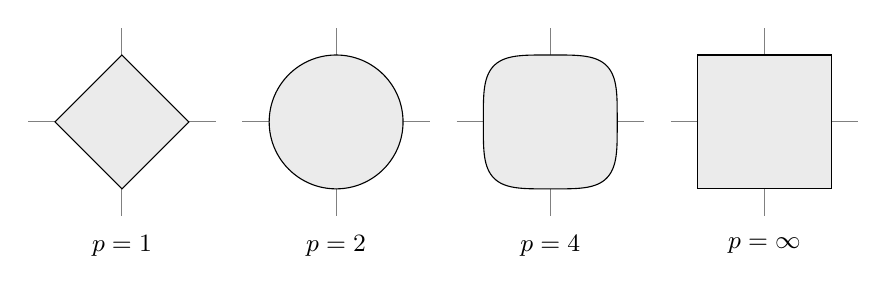
\begin{tikzpicture}[scale=0.85, every node/.style={font=\small}]
  \foreach \x/\lbl in {0/{$p = 1$}, 3.2/{$p = 2$}, 6.4/{$p = 4$}, 9.6/{$p = \infty$}} {
    \draw[black!50] (\x-1.4,0) -- (\x+1.4,0);
    \draw[black!50] (\x,-1.4) -- (\x,1.4);
    \node at (\x,-1.85) {\lbl};
  }
  \filldraw[fill=black!8] (1,0) -- (0,1) -- (-1,0) -- (0,-1) -- cycle;
  \filldraw[fill=black!8] (3.2,0) circle (1);
  \filldraw[fill=black!8, xshift=6.4cm] plot[domain=0:360, samples=120, smooth cycle]
    ({sign(cos(\x))*abs(cos(\x))^0.5}, {sign(sin(\x))*abs(sin(\x))^0.5});
  \filldraw[fill=black!8] (8.6,-1) rectangle (10.6,1);
\end{tikzpicture}

\small Unit balls of $\R^2$ in the $p$-norms. As $p$ grows, the ball grows from the diamond ($p = 1$) to the square ($p = \infty$).
\end{center}

The $2$-norm is the Euclidean length, and its unit ball is round. Since the balls are nested, the $p$-norms decrease as $p$ increases; \Cref{cor:pnorm-compare} below makes this precise, with constants depending on the dimension.

Aside from the $p$-norms, the most useful norms are the \emph{weighted norms}. Given any norm $\norm{\cdot}$ and a diagonal matrix $W = \diag(w_1, \dots, w_m)$ with all $w_i \ne 0$, we set
\begin{equation}
  \norm{\vec{x}}_W \doteq \norm{W\vec{x}}.
\end{equation}
For example, the weighted $2$-norm is $\norm{\vec{x}}_W = \left(\sum_i\abs{w_ix_i}^2\right)^{1/2}$, and its unit ball is an axis-aligned ellipse with semiaxes $1/\abs{w_i}$. More generally, $\norm{W\vec{x}}$ is a norm for \emph{any} nonsingular $W$: properties 2 and 3 are inherited from $\norm{\cdot}$ because $W$ is linear, and $\norm{W\vec{x}} = 0$ forces $W\vec{x} = \zerovec$, hence $\vec{x} = \zerovec$. Weighted norms are natural when the entries of $\vec{x}$ are measured in different units.

\subsection{Induced Matrix Norms}

An $m \times n$ matrix can be viewed as a vector in an $mn$-dimensional space, so any vector norm on $\K^{mn}$ measures the size of a matrix. More useful, however, are norms that measure what $A$ \emph{does} as a map from $\K^n$ to $\K^m$.

\begin{definition}[Induced Matrix Norm]
  \label{def:induced}
  Let $\norm{\cdot}_{(n)}$ and $\norm{\cdot}_{(m)}$ be norms on $\K^n$ and $\K^m$. The \emph{induced matrix norm} of $A \in \K^{m \times n}$ is the smallest $C$ such that $\norm{A\vec{x}}_{(m)} \le C\norm{\vec{x}}_{(n)}$ for all $\vec{x} \in \K^n$, that is,
  \begin{equation}
    \norm{A}_{(m,n)} \doteq \sup_{\vec{x} \ne \zerovec}\frac{\norm{A\vec{x}}_{(m)}}{\norm{\vec{x}}_{(n)}} = \sup_{\norm{\vec{x}}_{(n)} = 1}\norm{A\vec{x}}_{(m)}.
  \end{equation}
  When both norms are $p$-norms, we write $\norm{A}_p$.
\end{definition}

So $\norm{A}_{(m,n)}$ is the largest factor by which $A$ can stretch a vector. The two expressions agree by property 3 of \Cref{def:vector-norm}: scaling $\vec{x}$ does not change the ratio, so it suffices to look at unit vectors. In particular, $\norm{A}$ is determined by the image of the unit ball under $A$, which makes induced norms easy to visualize.

\begin{example}[A $2 \times 2$ Matrix in Three Norms]
  \label{ex:three-norms}
  Take
  \begin{equation}
    A = \begin{bmatrix} 1 & 2 \\ 0 & 2 \end{bmatrix}.
  \end{equation}
  Since $A$ is real, we may draw it as a map of $\R^2$. It sends $\vec{e}_1$ to its first column $(1, 0)^\T$ and $\vec{e}_2$ to its second column $(2, 2)^\T$. Mapping the unit balls of the $1$-, $2$-, and $\infty$-norms gives the following picture.

  \begin{center}
  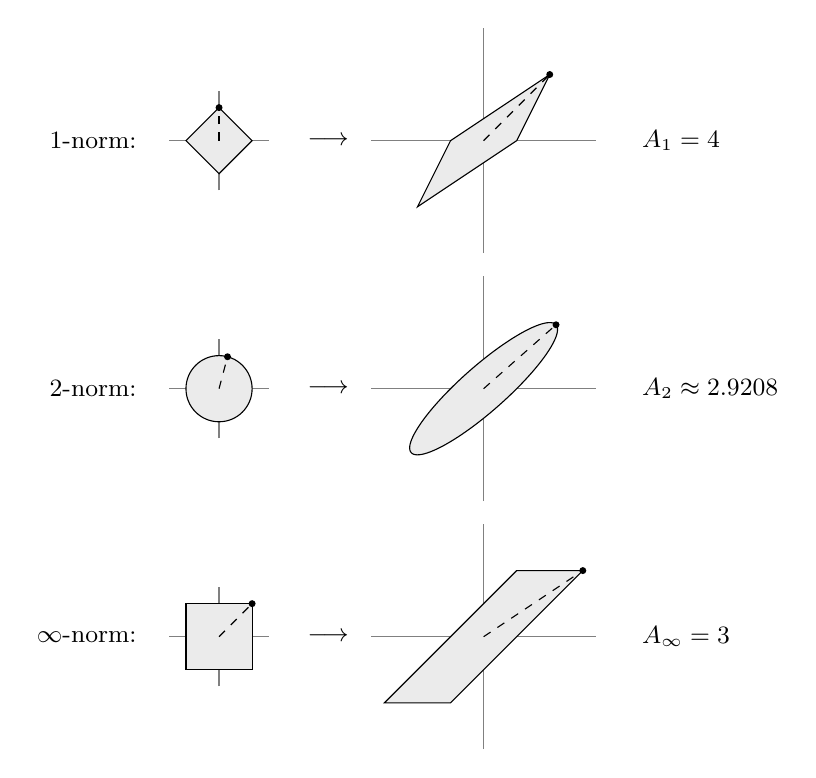
\begin{tikzpicture}[scale=0.42, every node/.style={font=\small}]
    \def\axes#1#2{\draw[black!50] (#1-#2,0) -- (#1+#2,0); \draw[black!50] (#1,-#2) -- (#1,#2);}
    % 1-norm
    \begin{scope}[yshift=0cm]
      \node[anchor=east] at (-2.2,0) {$1$-norm:};
      \axes{0}{1.5}
      \filldraw[fill=black!8] (1,0) -- (0,1) -- (-1,0) -- (0,-1) -- cycle;
      \draw[dashed] (0,0) -- (0,1); \fill (0,1) circle (3pt);
      \node at (3.3,0) {$\longrightarrow$};
      \axes{8}{3.4}
      \filldraw[fill=black!8, xshift=8cm] (1,0) -- (2,2) -- (-1,0) -- (-2,-2) -- cycle;
      \draw[dashed, xshift=8cm] (0,0) -- (2,2); \fill[xshift=8cm] (2,2) circle (3pt);
      \node[anchor=west] at (12.5,0) {$\norm{A}_1 = 4$};
    \end{scope}
    % 2-norm
    \begin{scope}[yshift=-7.5cm]
      \node[anchor=east] at (-2.2,0) {$2$-norm:};
      \axes{0}{1.5}
      \filldraw[fill=black!8] (0,0) circle (1);
      \draw[dashed] (0,0) -- (0.2567,0.9665); \fill (0.2567,0.9665) circle (3pt);
      \node at (3.3,0) {$\longrightarrow$};
      \axes{8}{3.4}
      \filldraw[fill=black!8, xshift=8cm] plot[domain=0:360, samples=100, smooth cycle]
        ({cos(\x) + 2*sin(\x)}, {2*sin(\x)});
      \draw[dashed, xshift=8cm] (0,0) -- (2.190,1.933); \fill[xshift=8cm] (2.190,1.933) circle (3pt);
      \node[anchor=west] at (12.5,0) {$\norm{A}_2 \approx 2.9208$};
    \end{scope}
    % infinity-norm
    \begin{scope}[yshift=-15cm]
      \node[anchor=east] at (-2.2,0) {$\infty$-norm:};
      \axes{0}{1.5}
      \filldraw[fill=black!8] (-1,-1) rectangle (1,1);
      \draw[dashed] (0,0) -- (1,1); \fill (1,1) circle (3pt);
      \node at (3.3,0) {$\longrightarrow$};
      \axes{8}{3.4}
      \filldraw[fill=black!8, xshift=8cm] (3,2) -- (1,2) -- (-3,-2) -- (-1,-2) -- cycle;
      \draw[dashed, xshift=8cm] (0,0) -- (3,2); \fill[xshift=8cm] (3,2) circle (3pt);
      \node[anchor=west] at (12.5,0) {$\norm{A}_\infty = 3$};
    \end{scope}
  \end{tikzpicture}

  \small Left: unit balls of $\R^2$. Right: their images under $A$. The dashed vectors are the ones that $A$ stretches the most in each norm.
  \end{center}

  In the $1$-norm, the most amplified unit vector is $\vec{e}_2$, which is mapped to $(2, 2)^\T$ with $1$-norm $4$. In the $\infty$-norm, it is $(1, 1)^\T$, which is mapped to $(3, 2)^\T$ with $\infty$-norm $3$. In the $2$-norm, the image of the unit circle is an ellipse, and $\norm{A}_2$ is the length of its longest semiaxis, about $2.9208$. This must be at least $\norm{A\vec{e}_2}_2 = \sqrt{8} \approx 2.8284$; the exact value is $\sigma_{\max}(A)$ by \Cref{thm:twonorm}.
\end{example}

\begin{example}[The $p$-Norm of a Diagonal Matrix]
  Let $D = \diag(d_1, \dots, d_m)$. For $1 \le p < \infty$,
  \begin{equation}
    \norm{D\vec{x}}_p^p = \sum_{i=1}^{m}\abs{d_ix_i}^p \le \left(\max_i\abs{d_i}\right)^p\norm{\vec{x}}_p^p,
  \end{equation}
  with equality for $\vec{x} = \vec{e}_i$ where $i$ maximizes $\abs{d_i}$; the case $p = \infty$ is the same argument with sums replaced by maxima. Hence $\norm{D}_p = \max_i\abs{d_i}$ for every $p$. Geometrically, $D$ maps the $2$-norm unit sphere to an ellipsoid with semiaxes $\abs{d_i}$, and $\norm{D}_2$ is the longest semiaxis. The SVD shows that \emph{every} matrix maps the unit sphere to an ellipsoid; only the axes may be rotated.
\end{example}

For $p = 1$ and $p = \infty$, the induced norm has a closed form in terms of the entries.

\begin{proposition}[The $1$- and $\infty$-Norms of a Matrix]
  \label{prop:one-inf-norm}
  Let $A \in \K^{m \times n}$ have columns $\vec{a}_1, \dots, \vec{a}_n$ and rows $\vec{\alpha}_1^\ast, \dots, \vec{\alpha}_m^\ast$. Then
  \begin{equation}
    \norm{A}_1 = \max_{1 \le j \le n}\norm{\vec{a}_j}_1 \quad\text{(maximum column sum)}, \qquad \norm{A}_\infty = \max_{1 \le i \le m}\norm{\vec{\alpha}_i}_1 \quad\text{(maximum row sum)}.
  \end{equation}
\end{proposition}

\begin{proof}
  For the $1$-norm, let $\norm{\vec{x}}_1 = 1$. By the triangle inequality,
  \begin{equation}
    \norm{A\vec{x}}_1 = \norm{\sum_{j=1}^{n}x_j\vec{a}_j}_1 \le \sum_{j=1}^{n}\abs{x_j}\norm{\vec{a}_j}_1 \le \max_j\norm{\vec{a}_j}_1,
  \end{equation}
  since the weights $\abs{x_j}$ sum to $1$. Taking $\vec{x} = \vec{e}_j$ for the column $j$ with the largest $1$-norm attains the bound.

  For the $\infty$-norm, let $\norm{\vec{x}}_\infty = 1$. Each entry of $A\vec{x}$ satisfies $\abs{(A\vec{x})_i} \le \sum_j\abs{A_{ij}}\abs{x_j} \le \norm{\vec{\alpha}_i}_1$, so $\norm{A\vec{x}}_\infty \le \max_i\norm{\vec{\alpha}_i}_1$. To attain it, pick the row $i$ with the largest $1$-norm and set $x_j = \overline{A_{ij}}/\abs{A_{ij}}$ (and $x_j = 1$ if $A_{ij} = 0$). Then $\norm{\vec{x}}_\infty = 1$ and $(A\vec{x})_i = \sum_j\abs{A_{ij}} = \norm{\vec{\alpha}_i}_1$.
\end{proof}

In the example above, the column sums are $1$ and $4$ and the row sums are $3$ and $2$, matching the picture. Both norms cost only $O(mn)$ operations, whereas $\norm{A}_2$ requires the largest singular value. Computing $\norm{A}_p$ for other $p$ is harder still.

\subsection{Cauchy--Schwarz and H\"older Inequalities}

To bound matrix norms when $p \ne 1, \infty$, we bound inner products by $p$-norms.

\begin{theorem}[H\"older and Cauchy--Schwarz Inequalities]
  \label{thm:holder}
  Let $1 \le p, q \le \infty$ with $1/p + 1/q = 1$. Then for all $\vec{x}, \vec{y} \in \K^m$,
  \begin{equation}
    \abs{\vec{x}^\ast\vec{y}} \le \norm{\vec{x}}_p\norm{\vec{y}}_q.
  \end{equation}
  The case $p = q = 2$ is the \emph{Cauchy--Schwarz inequality} $\abs{\vec{x}^\ast\vec{y}} \le \norm{\vec{x}}_2\norm{\vec{y}}_2$.
\end{theorem}

Both bounds are tight: for every $\vec{x}$ there is a $\vec{y} \ne \zerovec$ attaining equality. For Cauchy--Schwarz, $\vec{y} = \vec{x}$ works. Proofs can be found in any linear algebra text. These inequalities immediately give the $2$-norm of two simple kinds of matrices.

\begin{example}[The $2$-Norm of a Row Vector]
  Let $A = \vec{a}^\ast$ be a single row. By Cauchy--Schwarz, $\norm{A\vec{x}}_2 = \abs{\vec{a}^\ast\vec{x}} \le \norm{\vec{a}}_2\norm{\vec{x}}_2$, with equality for $\vec{x} = \vec{a}$. Hence $\norm{\vec{a}^\ast}_2 = \norm{\vec{a}}_2$.
\end{example}

\begin{example}[The $2$-Norm of an Outer Product]
  \label{ex:outer-norm}
  Let $A = \vec{u}\vec{v}^\ast$ with $\vec{u} \in \K^m$ and $\vec{v} \in \K^n$. For every $\vec{x} \in \K^n$,
  \begin{equation}
    \norm{A\vec{x}}_2 = \norm{\vec{u}(\vec{v}^\ast\vec{x})}_2 = \norm{\vec{u}}_2\abs{\vec{v}^\ast\vec{x}} \le \norm{\vec{u}}_2\norm{\vec{v}}_2\norm{\vec{x}}_2,
  \end{equation}
  with equality for $\vec{x} = \vec{v}$. Hence $\norm{\vec{u}\vec{v}^\ast}_2 = \norm{\vec{u}}_2\norm{\vec{v}}_2$. The Frobenius norm gives the same value: $\norm{\vec{u}\vec{v}^\ast}_F^2 = \sum_{i,j}\abs{u_i}^2\abs{v_j}^2 = \norm{\vec{u}}_2^2\norm{\vec{v}}_2^2$, consistent with item 3 of \Cref{prop:frobenius} for $r = 1$.
\end{example}

Cauchy--Schwarz also lets us compare the $p$-norms in a fixed dimension.

\begin{corollary}[Comparing $p$-Norms]
  \label{cor:pnorm-compare}
  For $\vec{x} \in \K^m$,
  \begin{equation}
    \norm{\vec{x}}_\infty \le \norm{\vec{x}}_2 \le \norm{\vec{x}}_1 \le \sqrt{m}\,\norm{\vec{x}}_2 \le m\norm{\vec{x}}_\infty,
  \end{equation}
  and for $A \in \K^{m \times n}$,
  \begin{equation}
    \frac{1}{\sqrt{n}}\norm{A}_\infty \le \norm{A}_2 \le \sqrt{m}\,\norm{A}_\infty, \qquad \frac{1}{\sqrt{m}}\norm{A}_1 \le \norm{A}_2 \le \sqrt{n}\,\norm{A}_1.
  \end{equation}
\end{corollary}

\begin{proof}
  The first two inequalities hold because $\max_i\abs{x_i}^2 \le \sum_i\abs{x_i}^2 \le \left(\sum_i\abs{x_i}\right)^2$. The third is Cauchy--Schwarz applied to the vector of the $\abs{x_i}$ and the all-ones vector, and the fourth is $\sum_i\abs{x_i}^2 \le m\max_i\abs{x_i}^2$.

  For the matrix bounds, chain the vector bounds through the definition. For instance,
  \begin{equation}
    \norm{A\vec{x}}_2 \le \sqrt{m}\,\norm{A\vec{x}}_\infty \le \sqrt{m}\,\norm{A}_\infty\norm{\vec{x}}_\infty \le \sqrt{m}\,\norm{A}_\infty\norm{\vec{x}}_2
  \end{equation}
  gives $\norm{A}_2 \le \sqrt{m}\,\norm{A}_\infty$, and $\norm{A\vec{x}}_\infty \le \norm{A\vec{x}}_2 \le \norm{A}_2\norm{\vec{x}}_2 \le \sqrt{n}\,\norm{A}_2\norm{\vec{x}}_\infty$ gives the other bound. The $1$-norm bounds follow in the same way.
\end{proof}

In particular, all $p$-norms agree up to factors that depend only on the dimension. Such factors are harmless in $O(\epsm)$ statements, so a method that is stable in one $p$-norm is stable in all of them.

\subsection{Bounding $\norm{AB}$}

\begin{proposition}[Submultiplicativity of Induced Norms]
  \label{prop:submult}
  Let $\norm{\cdot}_{(\ell)}$, $\norm{\cdot}_{(m)}$, $\norm{\cdot}_{(n)}$ be norms on $\K^\ell$, $\K^m$, $\K^n$, and let $A \in \K^{\ell \times m}$ and $B \in \K^{m \times n}$. Then
  \begin{equation}
    \norm{AB}_{(\ell,n)} \le \norm{A}_{(\ell,m)}\norm{B}_{(m,n)}.
  \end{equation}
\end{proposition}

\begin{proof}
  Apply the definition twice: $\norm{AB\vec{x}}_{(\ell)} \le \norm{A}_{(\ell,m)}\norm{B\vec{x}}_{(m)} \le \norm{A}_{(\ell,m)}\norm{B}_{(m,n)}\norm{\vec{x}}_{(n)}$.
\end{proof}

In particular, $\norm{A^k} \le \norm{A}^k$ for a square matrix in any induced norm. This is generally not an equality. For example, $A = \left[\begin{smallmatrix} 0 & 1 \\ 0 & 0 \end{smallmatrix}\right]$ has $\norm{A}_p = 1$ for every $p$, but $A^2 = 0$.

A related bound concerns eigenvalues. If $A\vec{x} = \lambda\vec{x}$ with $\vec{x} \ne \zerovec$, then $\abs{\lambda}\norm{\vec{x}} = \norm{A\vec{x}} \le \norm{A}\norm{\vec{x}}$. So the \emph{spectral radius} $\rho(A) \doteq \max\{\abs{\lambda} : \lambda \text{ an eigenvalue of } A\}$ satisfies
\begin{equation}
  \rho(A) \le \norm{A}
\end{equation}
in every induced norm. The same example shows that the inequality can be strict: $\rho(A) = 0$ but $\norm{A} = 1$.

\subsection{General Matrix Norms}

Matrix norms do not have to be induced by vector norms. In general, a \emph{matrix norm} is any function on $\K^{m \times n}$ that satisfies the three conditions of \Cref{def:vector-norm} on this $mn$-dimensional vector space:
\begin{equation}
  \norm{A} \ge 0 \text{ with equality only if } A = 0, \qquad \norm{A + B} \le \norm{A} + \norm{B}, \qquad \norm{\alpha A} = \abs{\alpha}\norm{A}.
\end{equation}
The most important matrix norm that is not induced by a vector norm is the Frobenius norm, the subject of \Cref{sec:frobenius}. Finally, the $2$-norm and the Frobenius norm are both invariant under multiplication by unitary matrices; this is \Cref{thm:unitary} below.

\section{Unitary Transformations}
\label{sec:unitary}

The error analysis of \Cref{ch:householder} uses one property of unitary matrices: they do not change the length of a vector. In this section we collect this and a few related facts, which we also use in \Cref{ch:ls,ch:qr}.

\begin{definition}[Unitary and Orthogonal Matrices]
  We say that a square matrix $Q \in \K^{m \times m}$ is \emph{unitary} if $Q^\ast Q = I$. When $\K = \R$, this condition reads $Q^\T Q = I$, and we call $Q$ \emph{orthogonal}. We say that a tall matrix $\hat{Q} \in \K^{m \times n}$ has \emph{orthonormal columns} if $\hat{Q}^\ast\hat{Q} = I_n$.
\end{definition}

The condition $Q^\ast Q = I$ just says that the columns of $Q$ are orthonormal. Since $Q$ is square, it also gives $Q^{-1} = Q^\ast$ and $QQ^\ast = I$. In particular, inverting a unitary matrix costs nothing: the solution of $Q\vec{x} = \vec{b}$ is $\vec{x} = Q^\ast\vec{b}$.

\begin{theorem}[Unitary Matrices Preserve the $2$-Norm]
  \label{thm:unitary}
  Let $Q \in \K^{m \times m}$ be unitary. Then for all $\vec{x}, \vec{y} \in \K^m$,
  \begin{equation}
    \ip{Q\vec{x}}{Q\vec{y}} = \ip{\vec{x}}{\vec{y}}, \qquad \norm{Q\vec{x}}_2 = \norm{\vec{x}}_2.
  \end{equation}
  As a consequence, for any $A \in \K^{m \times n}$ and unitary $U \in \K^{m \times m}$, $V \in \K^{n \times n}$:
  \begin{enumerate}
    \item $\norm{UAV}_2 = \norm{A}_2$ and $\norm{UAV}_F = \norm{A}_F$.
    \item $UAV$ has the same singular values as $A$. In particular, $\kappa_2(UAV) = \kappa_2(A)$.
    \item $\norm{Q}_2 = \norm{Q^{-1}}_2 = 1$ and $\kappa_2(Q) = 1$. All singular values of $Q$ are $1$, every eigenvalue of $Q$ satisfies $\abs{\lambda} = 1$, and $\abs{\det Q} = 1$.
  \end{enumerate}
\end{theorem}

\begin{proof}
  We have $\ip{Q\vec{x}}{Q\vec{y}} = \vec{x}^\ast Q^\ast Q\vec{y} = \vec{x}^\ast\vec{y}$. Taking $\vec{y} = \vec{x}$ gives $\norm{Q\vec{x}}_2 = \norm{\vec{x}}_2$.

  For item 1, the norm identity gives $\norm{UA\vec{x}}_2 = \norm{A\vec{x}}_2$ for every $\vec{x}$, so $\norm{UA}_2 = \norm{A}_2$. For the right factor, note that $\vec{y} = V\vec{x}$ runs over all unit vectors as $\vec{x}$ does, so
  \begin{equation}
    \norm{AV}_2 = \sup_{\norm{\vec{x}}_2 = 1}\norm{AV\vec{x}}_2 = \sup_{\norm{\vec{y}}_2 = 1}\norm{A\vec{y}}_2 = \norm{A}_2.
  \end{equation}
  The statement for the Frobenius norm is item 1 of \Cref{prop:frobenius}.

  For item 2, let $A = W\Sigma Z^\ast$ be an SVD. Then $UAV = (UW)\Sigma(V^\ast Z)^\ast$. Products of unitary matrices are unitary, so this is an SVD of $UAV$ with the same $\Sigma$.

  For item 3, $Q = Q \cdot I \cdot I^\ast$ is an SVD with $\Sigma = I$. If $Q\vec{x} = \lambda\vec{x}$ with $\vec{x} \ne \zerovec$, then $\norm{\vec{x}}_2 = \norm{Q\vec{x}}_2 = \abs{\lambda}\norm{\vec{x}}_2$, so $\abs{\lambda} = 1$. Finally, $\abs{\det Q}^2 = \det(Q^\ast Q) = \det I = 1$.
\end{proof}

The converse is also true: if $\norm{Q\vec{x}}_2 = \norm{\vec{x}}_2$ for every $\vec{x}$, then $Q$ is unitary. (One recovers inner products from norms by the polarization identity.) In other words, unitary matrices are exactly the linear maps that preserve lengths. Geometrically, they are rotations and reflections.

\subsection{Examples}

Several matrices we have already seen are unitary.
\begin{itemize}
  \item \emph{Householder reflectors} $F = I - 2\vec{v}\vec{v}^\ast/(\vec{v}^\ast\vec{v})$. They are Hermitian, satisfy $F^2 = I$, and have $\det F = -1$.
  \item \emph{Givens rotations} (\Cref{ch:qr}). They have $\det = 1$ and change only two coordinates.
  \item \emph{Permutation matrices}. So the row swaps of partial pivoting (\Cref{ch:pivoting}) do not change any norms, and all of the instability of LU comes from the triangular factors.
  \item \emph{Diagonal matrices} $D = \diag(d_1, \dots, d_m)$ with $\abs{d_i} = 1$. These describe exactly the freedom in the QR factorization, since $A = (QD)(D^\ast R)$. The condition $r_{jj} > 0$ removes this freedom (\Cref{thm:qr-unique}).
\end{itemize}

\subsection{Tall Matrices with Orthonormal Columns}

Now let $\hat{Q} \in \K^{m \times n}$ with $m > n$ have orthonormal columns. The same one-line proof shows that $\norm{\hat{Q}\vec{x}}_2 = \norm{\vec{x}}_2$, and hence, as in item 1 of \Cref{thm:unitary}, $\norm{\hat{Q}B}_2 = \norm{B}_2$ and $\norm{\hat{Q}B}_F = \norm{B}_F$ for every $B \in \K^{n \times p}$. Taking conjugate transposes, the same holds for multiplication on the right by a matrix with orthonormal rows. However, $\hat{Q}^\ast$ does \emph{not} preserve lengths. The matrix $\hat{Q}\hat{Q}^\ast$ is not the identity; it is the orthogonal projector onto $\range(\hat{Q})$. So $\norm{\hat{Q}^\ast\vec{y}}_2 \le \norm{\vec{y}}_2$, with equality only if $\vec{y} \in \range(\hat{Q})$.

This is exactly what makes QR useful for least squares. Take a full QR factorization $A = QR = \begin{bmatrix} \hat{Q} & \hat{Q}_\perp \end{bmatrix}\begin{bmatrix} \hat{R} \\ 0 \end{bmatrix}$. Since $Q^\ast$ preserves lengths, we can apply it inside the norm:
\begin{equation}
  \norm{A\vec{x} - \vec{b}}_2^2 = \norm{Q^\ast(A\vec{x} - \vec{b})}_2^2 = \norm{\hat{R}\vec{x} - \hat{Q}^\ast\vec{b}}_2^2 + \norm{\hat{Q}_\perp^\ast\vec{b}}_2^2.
\end{equation}
The second term does not depend on $\vec{x}$. So the minimizer solves $\hat{R}\vec{x} = \hat{Q}^\ast\vec{b}$, and the minimal residual is $\norm{\hat{Q}_\perp^\ast\vec{b}}_2$ (compare \Cref{ch:ls}).

\subsection{Why Unitary Transformations Are Good for Computation}

\begin{enumerate}
  \item \emph{One step does not amplify errors.} In \Cref{thm:product-error} we have $\kappa(Q_k) = 1$, so each step has relative backward error $O(\epsm)$ with no extra factor.
  \item \emph{Many steps do not amplify errors.} A product of unitary matrices is unitary. So when we pull an error back through all the previous steps, its size does not change. The backward errors of $n$ steps add up to $O(n\epsm)$ instead of multiplying (see \Cref{sec:hh-supp}).
  \item \emph{No element growth.} Every intermediate matrix has the same $2$-norm as $A$, so there is nothing like the growth factor of LU. Compare this with \Cref{ex:linv}: a triangular matrix with entries bounded by $1$ can still have an exponentially large inverse, while $\norm{Q^{-1}}_2 = \norm{Q}_2 = 1$ always.
  \item \emph{Errors look the same before and after.} An error of size $\delta$ in $\vec{x}$ is an error of size $\delta$ in $Q\vec{x}$. So we can move errors between the input and the output without losing anything.
\end{enumerate}

Note that this invariance holds for the $2$-norm and the Frobenius norm, but not for other norms. For example, rotating $\vec{e}_1$ by $45^\circ$ gives $(1/\sqrt{2}, 1/\sqrt{2})^\T$, whose $\infty$-norm is $1/\sqrt{2}$ and whose $1$-norm is $\sqrt{2}$. This is why stability results for orthogonal methods are stated in the $2$-norm. In other norms they still hold, but with extra constants that depend on the dimension.

As a final note, everything above assumes that the transformation is \emph{exactly} unitary. A matrix that we compute column by column, such as the $\hat{Q}$ of modified Gram--Schmidt, is only unitary up to $O(\epsm\kappa(A))$, and it loses these advantages to the same extent. Householder's $Q$ is different. Each reflector built from a computed vector $\tilde{\vec{v}}_k$ is exactly unitary, so rounding errors only change \emph{which} unitary matrix we get, not \emph{whether} it is unitary (\Cref{ch:qr}).

\section{The $2$-Norm, Singular Values, and Condition Numbers}
\label{sec:twonorm}

Most error bounds in this course are stated in the $2$-norm. Here we record how it is expressed through the SVD; these facts are proved in Homework 1, Problem 3.

\begin{definition}[Induced $2$-Norm]
  The \emph{$2$-norm} of $A \in \K^{m \times n}$ is the matrix norm induced by the vector $2$-norm (\Cref{def:induced}),
  \begin{equation}
    \norm{A}_2 \doteq \sup_{\vec{x} \ne \zerovec}\frac{\norm{A\vec{x}}_2}{\norm{\vec{x}}_2}.
  \end{equation}
\end{definition}

\begin{theorem}[The $2$-Norm Through the SVD]
  \label{thm:twonorm}
  Let $A \in \K^{m \times n}$ have singular values $\sigma_{\max} = \sigma_1 \ge \cdots \ge \sigma_{\min(m,n)} = \sigma_{\min}$. Then:
  \begin{enumerate}
    \item $\norm{A}_2 = \sigma_{\max}$.
    \item If $m \ge n$, then $\norm{A\vec{x}}_2 \ge \sigma_{\min}\norm{\vec{x}}_2$ for all $\vec{x}$, with equality for the last right singular vector.
    \item If $A$ is square and invertible, then $\norm{A^{-1}}_2 = 1/\sigma_{\min}$, and hence
    \begin{equation}
      \kappa_2(A) \doteq \norm{A}_2\norm{A^{-1}}_2 = \frac{\sigma_{\max}}{\sigma_{\min}}.
    \end{equation}
  \end{enumerate}
\end{theorem}

\begin{proof}
  Take an SVD $A = U\Sigma V^\ast$ and put $\vec{y} = V^\ast\vec{x}$. Since $U$ and $V$ are unitary (\Cref{thm:unitary}), $\norm{A\vec{x}}_2 = \norm{\Sigma\vec{y}}_2$ and $\norm{\vec{y}}_2 = \norm{\vec{x}}_2$. Now
  \begin{equation}
    \norm{\Sigma\vec{y}}_2^2 = \sum_{i}\sigma_i^2\abs{y_i}^2.
  \end{equation}
  This is at most $\sigma_{\max}^2\norm{\vec{y}}_2^2$, with equality for $\vec{y} = \vec{e}_1$, which gives item 1. If $m \ge n$, the sum runs over all $n$ entries of $\vec{y}$, so it is at least $\sigma_{\min}^2\norm{\vec{y}}_2^2$, with equality for $\vec{y} = \vec{e}_n$; this gives item 2. For item 3, $A^{-1} = V\Sigma^{-1}U^\ast$ is an SVD up to reordering, so the singular values of $A^{-1}$ are the $1/\sigma_i$, and the largest of them is $1/\sigma_{\min}$.
\end{proof}

For a tall matrix with full column rank we \emph{define} $\kappa_2(A) \doteq \sigma_{\max}/\sigma_{\min}$; this is the condition number that governs least squares (\Cref{ch:ls}). In both cases, $\kappa_2(A)$ is the worst-case condition number of the map $\vec{x} \mapsto A\vec{x}$ from \Cref{ch:fp}:
\begin{equation}
  \sup_{\vec{x} \ne \zerovec}\frac{\norm{A}_2\norm{\vec{x}}_2}{\norm{A\vec{x}}_2} = \frac{\sigma_{\max}}{\sigma_{\min}},
\end{equation}
since $\norm{A\vec{x}}_2/\norm{\vec{x}}_2$ is smallest, equal to $\sigma_{\min}$, for the last right singular vector. In words, $\kappa_2(A)$ is the ratio of the largest to the smallest stretching factor of $A$.

\section{The Frobenius Norm}
\label{sec:frobenius}

In \Cref{ch:householder} we bounded $\norm{L}_2$ through the Frobenius norm. It is often the easiest matrix norm to compute and to estimate.

\begin{definition}[Frobenius Norm]
  The \emph{Frobenius norm} of $A \in \K^{m \times n}$ is
  \begin{equation}
    \norm{A}_F \doteq \left(\sum_{i=1}^{m}\sum_{j=1}^{n}\abs{A_{ij}}^2\right)^{1/2}.
  \end{equation}
\end{definition}

In other words, $\norm{A}_F$ is the Euclidean norm of $A$ if we stack its columns into one long vector of length $mn$. Equivalently, $\norm{A}_F^2 = \sum_j\norm{\vec{a}_j}_2^2$ is the sum of the squared column norms. These squared column norms are exactly the diagonal entries of $A^\ast A$, and the squared row norms are the diagonal entries of $AA^\ast$, so
\begin{equation}
  \norm{A}_F^2 = \operatorname{trace}(A^\ast A) = \operatorname{trace}(AA^\ast).
\end{equation}

\begin{proposition}[Properties of the Frobenius Norm]
  \label{prop:frobenius}
  Let $A \in \K^{m \times n}$ have rank $r$ and singular values $\sigma_1 \ge \cdots \ge \sigma_r > 0$. Then:
  \begin{enumerate}
    \item \emph{Unitary invariance.} $\norm{UAV}_F = \norm{A}_F$ for all unitary $U \in \K^{m \times m}$ and $V \in \K^{n \times n}$.
    \item \emph{Singular values.} $\norm{A}_F = \left(\sigma_1^2 + \cdots + \sigma_r^2\right)^{1/2}$.
    \item \emph{Comparison with the $2$-norm.} $\norm{A}_2 \le \norm{A}_F \le \sqrt{r}\,\norm{A}_2 \le \sqrt{\min(m, n)}\,\norm{A}_2$.
    \item \emph{Compatibility and submultiplicativity.} $\norm{A\vec{x}}_2 \le \norm{A}_F\norm{\vec{x}}_2$, and $\norm{AB}_F \le \norm{A}_2\norm{B}_F \le \norm{A}_F\norm{B}_F$.
    \item \emph{Only absolute values matter.} $\norm{A}_F = \norm{\abs{A}}_F$, and if $\abs{A} \le \abs{B}$ entrywise, then $\norm{A}_F \le \norm{B}_F$.
  \end{enumerate}
\end{proposition}

\begin{proof}
  For item 1, using $U^\ast U = I$ and the cyclic property of the trace,
  \begin{equation}
    \norm{UAV}_F^2 = \operatorname{trace}(V^\ast A^\ast U^\ast UAV) = \operatorname{trace}(V^\ast A^\ast AV) = \operatorname{trace}(A^\ast A) = \norm{A}_F^2.
  \end{equation}
  For item 2, take an SVD $A = U\Sigma V^\ast$. By item 1, $\norm{A}_F = \norm{\Sigma}_F = (\sum_i\sigma_i^2)^{1/2}$.

  For item 3, use item 2 and $\norm{A}_2 = \sigma_1$: we have $\sigma_1^2 \le \sum_i\sigma_i^2 \le r\sigma_1^2$.

  For item 4, let $\vec{\alpha}_i^\ast$ be the $i$-th row of $A$. By the Cauchy--Schwarz inequality, $\abs{\vec{\alpha}_i^\ast\vec{x}}^2 \le \norm{\vec{\alpha}_i}_2^2\norm{\vec{x}}_2^2$. Summing over $i$ gives $\norm{A\vec{x}}_2^2 \le \norm{A}_F^2\norm{\vec{x}}_2^2$. For the product, apply $\norm{A\vec{b}_j}_2 \le \norm{A}_2\norm{\vec{b}_j}_2$ to each column $\vec{b}_j$ of $B$ and sum the squares. The last inequality then follows from $\norm{A}_2 \le \norm{A}_F$.

  Item 5 follows directly from the definition.
\end{proof}

Note that the Frobenius norm is \emph{not} induced by any vector norm. Every induced norm satisfies $\norm{I} = \sup_{\vec{x} \ne \zerovec}\norm{\vec{x}}/\norm{\vec{x}} = 1$, but $\norm{I_n}_F = \sqrt{n}$. Still, by item 4 it is compatible with the Euclidean norm on vectors.

\subsection{Why It Is Useful in Error Analysis}

\begin{itemize}
  \item \emph{It is cheap.} Computing $\norm{A}_F$ takes $O(mn)$ operations, while $\norm{A}_2 = \sigma_1$ requires the SVD (or an estimate of it). By item 3, the two norms differ by at most a factor of $\sqrt{\min(m, n)}$, and such dimension-dependent constants do not matter in $O(\epsm)$ statements.
  \item \emph{It turns entrywise bounds into norm bounds.} The backward error of LU from \Cref{ch:pivoting} satisfies $\abs{E} \le m\epsm\abs{L}\abs{U}$. By items 5 and 4,
  \begin{equation}
    \norm{E}_F \le m\epsm\norm{\abs{L}\abs{U}}_F \le m\epsm\norm{L}_F\norm{U}_F.
  \end{equation}
  With partial pivoting, $\norm{L}_F \le m$ (\Cref{ch:householder}), so everything depends on $\norm{U}_F$, i.e., on the growth factor.
  \item \emph{It is unitarily invariant.} Just like the $2$-norm, the Frobenius norm of an error does not change under orthogonal transformations such as Householder reflectors.
\end{itemize}

\subsection{Low-Rank Approximation}

Since $\norm{A - B}_F^2 = \sum_{i,j}\abs{A_{ij} - B_{ij}}^2$ is a sum of squared entrywise errors, approximating a matrix in the Frobenius norm is a least squares problem. The Eckart--Young theorem also holds in this norm: the truncated SVD $A_k = \sum_{i \le k}\sigma_i\vec{u}_i\vec{v}_i^\ast$ satisfies
\begin{equation}
  \min_{\rank(B) \le k}\norm{A - B}_F = \norm{A - A_k}_F = \left(\sigma_{k+1}^2 + \cdots + \sigma_r^2\right)^{1/2}.
\end{equation}
In the $2$-norm, the corresponding error is $\norm{A - A_k}_2 = \sigma_{k+1}$~\cite[\S3.2.3]{Demmel}. We will come back to this when the course covers low-rank approximation.

